% -*- Mode:TeX -*-

%% IMPORTANT: The official thesis specifications are available at:
%%            http://libraries.mit.edu/archives/thesis-specs/
%%
%%            Please verify your thesis' formatting and copyright
%%            assignment before submission.  If you notice any
%%            discrepancies between these templates and the 
%%            MIT Libraries' specs, please let us know
%%            by e-mailing thesis@mit.edu

%% The documentclass options along with the pagestyle can be used to generate
%% a technical report, a draft copy, or a regular thesis.  You may need to
%% re-specify the pagestyle after you \include  cover.tex.  For more
%% information, see the first few lines of mitthesis.cls. 

%\documentclass[12pt,vi,twoside]{mitthesis}
%%
%%  If you want your thesis copyright to you instead of MIT, use the
%%  ``vi'' option, as above.
%%
%\documentclass[12pt,twoside,leftblank]{mitthesis}
%%
%% If you want blank pages before new chapters to be labelled ``This
%% Page Intentionally Left Blank'', use the ``leftblank'' option, as
%% above. 


\documentclass[12pt,singlespace]{mitthesis}
\usepackage{lgrind}
\pagestyle{plain}

%% This bit allows you to either specify only the files which you wish to
%% process, or `all' to process all files which you \include.
%% Krishna Sethuraman (1990).

\typein [\files]{Enter file names to process, (chap1,chap2 ...), or `all' to
process all files:}
\def\all{all}
\ifx\files\all \typeout{Including all files.} \else \typeout{Including only \files.} \includeonly{\files} \fi

\renewcommand*\thesection{\arabic{section}}

\begin{document}

% -*-latex-*-
% 
% For questions, comments, concerns or complaints:
% thesis@mit.edu
% 
%
% $Log: cover.tex,v $
% Revision 1.8  2008/05/13 15:02:15  jdreed
% Degree month is June, not May.  Added note about prevdegrees.
% Arthur Smith's title updated
%
% Revision 1.7  2001/02/08 18:53:16  boojum
% changed some \newpages to \cleardoublepages
%
% Revision 1.6  1999/10/21 14:49:31  boojum
% changed comment referring to documentstyle
%
% Revision 1.5  1999/10/21 14:39:04  boojum
% *** empty log message ***
%
% Revision 1.4  1997/04/18  17:54:10  othomas
% added page numbers on abstract and cover, and made 1 abstract
% page the default rather than 2.  (anne hunter tells me this
% is the new institute standard.)
%
% Revision 1.4  1997/04/18  17:54:10  othomas
% added page numbers on abstract and cover, and made 1 abstract
% page the default rather than 2.  (anne hunter tells me this
% is the new institute standard.)
%
% Revision 1.3  93/05/17  17:06:29  starflt
% Added acknowledgements section (suggested by tompalka)
% 
% Revision 1.2  92/04/22  13:13:13  epeisach
% Fixes for 1991 course 6 requirements
% Phrase "and to grant others the right to do so" has been added to 
% permission clause
% Second copy of abstract is not counted as separate pages so numbering works
% out
% 
% Revision 1.1  92/04/22  13:08:20  epeisach

% NOTE:
% These templates make an effort to conform to the MIT Thesis specifications,
% however the specifications can change.  We recommend that you verify the
% layout of your title page with your thesis advisor and/or the MIT 
% Libraries before printing your final copy.
\title{The Aerodynamics of Paper Airplanes}

\author{Han Gao and Daniel Jeng}
% If you wish to list your previous degrees on the cover page, use the 
% previous degrees command:
%       \prevdegrees{A.A., Harvard University (1985)}
% You can use the \\ command to list multiple previous degrees
%       \prevdegrees{B.S., University of California (1978) \\
%                    S.M., Massachusetts Institute of Technology (1981)}
\department{Department of Electrical Engineering and Computer Science}

% If the thesis is for two degrees simultaneously, list them both
% separated by \and like this:
% \degree{Doctor of Philosophy \and Master of Science}
\degree{Bachelor of Science in Computer Science and Engineering}

% As of the 2007-08 academic year, valid degree months are September, 
% February, or June.  The default is June.
\degreemonth{June}
\degreeyear{1990}
\thesisdate{May 18, 1990}

%% By default, the thesis will be copyrighted to MIT.  If you need to copyright
%% the thesis to yourself, just specify the `vi' documentclass option.  If for
%% some reason you want to exactly specify the copyright notice text, you can
%% use the \copyrightnoticetext command.  
%\copyrightnoticetext{\copyright IBM, 1990.  Do not open till Xmas.}

% If there is more than one supervisor, use the \supervisor command
% once for each.
\supervisor{William J. Dally}{Associate Professor}

% This is the department committee chairman, not the thesis committee
% chairman.  You should replace this with your Department's Committee
% Chairman.
\chairman{Arthur C. Smith}{Chairman, Department Committee on Graduate Theses}

% If you wish to list your previous degrees on the cover page, use the 
% previous degrees command:
%       \prevdegrees{A.A., Harvard University (1985)}
% You can use the \\ command to list multiple previous degrees
%       \prevdegrees{B.S., University of California (1978) \\
%                    S.M., Massachusetts Institute of Technology (1981)}

% Make the titlepage based on the above information.  If you need
% something special and can't use the standard form, you can specify
% the exact text of the titlepage yourself.  Put it in a titlepage
% environment and leave blank lines where you want vertical space.
% The spaces will be adjusted to fill the entire page.  The dotted
% lines for the signatures are made with the \signature command.
\maketitle

% The abstractpage environment sets up everything on the page except
% the text itself.  The title and other header material are put at the
% top of the page, and the supervisors are listed at the bottom.  A
% new page is begun both before and after.  Of course, an abstract may
% be more than one page itself.  If you need more control over the
% format of the page, you can use the abstract environment, which puts
% the word "Abstract" at the beginning and single spaces its text.

%% You can either \input (*not* \include) your abstract file, or you can put
%% the text of the abstract directly between the \begin{abstractpage} and
%% \end{abstractpage} commands.

% First copy: start a new page, and save the page number.
% \cleardoublepage
% Uncomment the next line if you do NOT want a page number on your
% abstract and acknowledgments pages.
% \pagestyle{empty}
\setcounter{savepage}{\thepage}
\begin{abstractpage}
% $Log: abstract.tex,v $
% Revision 1.1  93/05/14  14:56:25  starflt
% Initial revision
% 
% Revision 1.1  90/05/04  10:41:01  lwvanels
% Initial revision
% 
%
%% The text of your abstract and nothing else (other than comments) goes here.
%% It will be single-spaced and the rest of the text that is supposed to go on
%% the abstract page will be generated by the abstractpage environment.  This
%% file should be \input (not \include 'd) from cover.tex.
In this paper we will explore the validity of drag and lift formulas on 
paper airplanes. We will construct airplanes of different sizes and geometries 
and calculate their theoretical drag and lift. We will perform experiments to
determine time of flight in order to compare them to our theoretical results.
Lastly we will also perform experiments to determine the stability of the airplane.

\end{abstractpage}

% Additional copy: start a new page, and reset the page number.  This way,
% the second copy of the abstract is not counted as separate pages.
% Uncomment the next 6 lines if you need two copies of the abstract
% page.
% \setcounter{page}{\thesavepage}
% \begin{abstractpage}
% % $Log: abstract.tex,v $
% Revision 1.1  93/05/14  14:56:25  starflt
% Initial revision
% 
% Revision 1.1  90/05/04  10:41:01  lwvanels
% Initial revision
% 
%
%% The text of your abstract and nothing else (other than comments) goes here.
%% It will be single-spaced and the rest of the text that is supposed to go on
%% the abstract page will be generated by the abstractpage environment.  This
%% file should be \input (not \include 'd) from cover.tex.
In this paper we will explore the validity of drag and lift formulas on 
paper airplanes. We will construct airplanes of different sizes and geometries 
and calculate their theoretical drag and lift. We will perform experiments to
determine time of flight in order to compare them to our theoretical results.
Lastly we will also perform experiments to determine the stability of the airplane.

% \end{abstractpage}


%%%%%%%%%%%%%%%%%%%%%%%%%%%%%%%%%%%%%%%%%%%%%%%%%%%%%%%%%%%%%%%%%%%%%%
% -*-latex-*-

% Some departments (e.g. 5) require an additional signature page.  See
% signature.tex for more information and uncomment the following line if
% applicable.
% % -*- Mode:TeX -*-
%
% Some departments (e.g. Chemistry) require an additional cover page
% with signatures of the thesis committee.  Please check with your
% thesis advisor or other appropriate person to determine if such a 
% page is required for your thesis.  
%
% If you choose not to use the "titlepage" environment, a \newpage
% commands, and several \vspace{\fill} commands may be necessary to
% achieve the required spacing.  The \signature command is defined in
% the "mitthesis" class
%
% The following sample appears courtesy of Ben Kaduk <kaduk@mit.edu> and
% was used in his June 2012 doctoral thesis in Chemistry. 

\begin{titlepage}
\begin{large}
This doctoral thesis has been examined by a Committee of the Department
of Chemistry as follows:

\signature{Professor Jianshu Cao}{Chairman, Thesis Committee \\
   Professor of Chemistry}

\signature{Professor Troy Van Voorhis}{Thesis Supervisor \\
   Associate Professor of Chemistry}

\signature{Professor Robert W. Field}{Member, Thesis Committee \\
   Haslam and Dewey Professor of Chemistry}
\end{large}
\end{titlepage}


%\pagestyle{plain}
%   % -*- Mode:TeX -*-
%% This file simply contains the commands that actually generate the table of
%% contents and lists of figures and tables.  You can omit any or all of
%% these files by simply taking out the appropriate command.  For more
%% information on these files, see appendix C.3.3 of the LaTeX manual. 
\tableofcontents
\newpage
\listoffigures
\newpage
\listoftables


%% This is an example first chapter.  You should put chapter/appendix that you
%% write into a separate file, and add a line \include{yourfilename} to
%% main.tex, where `yourfilename.tex' is the name of the chapter/appendix file.
%% You can process specific files by typing their names in at the 
%% \files=
%% prompt when you run the file main.tex through LaTeX.
\chapter{Introduction}

Micro-optimization is a technique to reduce the overall operation count of
floating point operations.  In a standard floating point unit, floating
point operations are fairly high level, such as ``multiply'' and ``add'';
in a micro floating point unit ($\mu$FPU), these have been broken down into
their constituent low-level floating point operations on the mantissas and
exponents of the floating point numbers.

Chapter two describes the architecture of the $\mu$FPU unit, and the
motivations for the design decisions made.

Chapter three describes the design of the compiler, as well as how the
optimizations discussed in section~\ref{ch1:opts} were implemented.

Chapter four describes the purpose of test code that was compiled, and which
statistics were gathered by running it through the simulator.  The purpose
is to measure what effect the micro-optimizations had, compared to
unoptimized code.  Possible future expansions to the project are also
discussed.

\section{Motivations for micro-optimization}

The idea of micro-optimization is motivated by the recent trends in computer
architecture towards low-level parallelism and small, pipelineable
instruction sets \cite{patterson:risc,rad83}.  By getting rid of more
complex instructions and concentrating on optimizing frequently used
instructions, substantial increases in performance were realized.

Another important motivation was the trend towards placing more of the
burden of performance on the compiler.  Many of the new architectures depend
on an intelligent, optimizing compiler in order to realize anywhere near
their peak performance
\cite{ellis:bulldog,pet87,coutant:precision-compilers}.  In these cases, the
compiler not only is responsible for faithfully generating native code to
match the source language, but also must be aware of instruction latencies,
delayed branches, pipeline stages, and a multitude of other factors in order
to generate fast code \cite{gib86}.

Taking these ideas one step further, it seems that the floating point
operations that are normally single, large instructions can be further broken
down into smaller, simpler, faster instructions, with more control in the
compiler and less in the hardware.  This is the idea behind a
micro-optimizing FPU; break the floating point instructions down into their
basic components and use a small, fast implementation, with a large part of
the burden of hardware allocation and optimization shifted towards
compile-time.

Along with the hardware speedups possible by using a $\mu$FPU, there are
also optimizations that the compiler can perform on the code that is
generated.  In a normal sequence of floating point operations, there are
many hidden redundancies that can be eliminated by allowing the compiler to
control the floating point operations down to their lowest level.  These
optimizations are described in detail in section~\ref{ch1:opts}.

\section{Description of micro-optimization}\label{ch1:opts}

In order to perform a sequence of floating point operations, a normal FPU
performs many redundant internal shifts and normalizations in the process of
performing a sequence of operations.  However, if a compiler can
decompose the floating point operations it needs down to the lowest level,
it then can optimize away many of these redundant operations.  

If there is some additional hardware support specifically for
micro-optimization, there are additional optimizations that can be
performed.  This hardware support entails extra ``guard bits'' on the
standard floating point formats, to allow several unnormalized operations to
be performed in a row without the loss information\footnote{A description of
the floating point format used is shown in figures~\ref{exponent-format}
and~\ref{mantissa-format}.}.  A discussion of the mathematics behind
unnormalized arithmetic is in appendix~\ref{unnorm-math}.

The optimizations that the compiler can perform fall into several categories:

\subsection{Post Multiply Normalization}

When more than two multiplications are performed in a row, the intermediate
normalization of the results between multiplications can be eliminated.
This is because with each multiplication, the mantissa can become
denormalized by at most one bit.  If there are guard bits on the mantissas
to prevent bits from ``falling off'' the end during multiplications, the
normalization can be postponed until after a sequence of several
multiplies\footnote{Using unnormalized numbers for math is not a new idea; a
good example of it is the Control Data CDC 6600, designed by Seymour Cray.
\cite{thornton:cdc6600} The CDC 6600 had all of its instructions performing
unnormalized arithmetic, with a separate {\tt NORMALIZE} instruction.}.

% This is an example of how you would use tgrind to include an example
% of source code; it is commented out in this template since the code
% example file does not exist.  To use it, you need to remove the '%' on the
% beginning of the line, and insert your own information in the call.
%
%\tagrind[htbp]{code/pmn.s.tex}{Post Multiply Normalization}{opt:pmn}

As you can see, the intermediate results can be multiplied together, with no
need for intermediate normalizations due to the guard bit.  It is only at
the end of the operation that the normalization must be performed, in order
to get it into a format suitable for storing in memory\footnote{Note that
for purposed of clarity, the pipeline delays were considered to be 0, and
the branches were not delayed.}.

\subsection{Block Exponent}

In a unoptimized sequence of additions, the sequence of operations is as
follows for each pair of numbers ($m_1$,$e_1$) and ($m_2$,$e_2$).
\begin{enumerate}
  \item Compare $e_1$ and $e_2$.
  \item Shift the mantissa associated with the smaller exponent $|e_1-e_2|$
        places to the right.
  \item Add $m_1$ and $m_2$.
  \item Find the first one in the resulting mantissa.
  \item Shift the resulting mantissa so that normalized
  \item Adjust the exponent accordingly.
\end{enumerate}

Out of 6 steps, only one is the actual addition, and the rest are involved
in aligning the mantissas prior to the add, and then normalizing the result
afterward.  In the block exponent optimization, the largest mantissa is
found to start with, and all the mantissa's shifted before any additions
take place.  Once the mantissas have been shifted, the additions can take
place one after another\footnote{This requires that for n consecutive
additions, there are $\log_{2}n$ high guard bits to prevent overflow.  In
the $\mu$FPU, there are 3 guard bits, making up to 8 consecutive additions
possible.}.  An example of the Block Exponent optimization on the expression
X = A + B + C is given in figure~\ref{opt:be}.

% This is an example of how you would use tgrind to include an example
% of source code; it is commented out in this template since the code
% example file does not exist.  To use it, you need to remove the '%' on the
% beginning of the line, and insert your own information in the call.
%
%\tgrind[htbp]{code/be.s.tex}{Block Exponent}{opt:be}

\section{Integer optimizations}

As well as the floating point optimizations described above, there are
also integer optimizations that can be used in the $\mu$FPU.  In concert
with the floating point optimizations, these can provide a significant
speedup.  

\subsection{Conversion to fixed point}

Integer operations are much faster than floating point operations; if it is
possible to replace floating point operations with fixed point operations,
this would provide a significant increase in speed.

This conversion can either take place automatically or or based on a
specific request from the programmer.  To do this automatically, the
compiler must either be very smart, or play fast and loose with the accuracy
and precision of the programmer's variables.  To be ``smart'', the computer
must track the ranges of all the floating point variables through the
program, and then see if there are any potential candidates for conversion
to floating point.  This technique is discussed further in
section~\ref{range-tracking}, where it was implemented.

The other way to do this is to rely on specific hints from the programmer
that a certain value will only assume a specific range, and that only a
specific precision is desired.  This is somewhat more taxing on the
programmer, in that he has to know the ranges that his values will take at
declaration time (something normally abstracted away), but it does provide
the opportunity for fine-tuning already working code.

Potential applications of this would be simulation programs, where the
variable represents some physical quantity; the constraints of the physical
system may provide bounds on the range the variable can take.
\subsection{Small Constant Multiplications}

One other class of optimizations that can be done is to replace
multiplications by small integer constants into some combination of
additions and shifts.  Addition and shifting can be significantly faster
than multiplication.  This is done by using some combination of
\begin{eqnarray*}
a_i & = & a_j + a_k \\
a_i & = & 2a_j + a_k \\
a_i & = & 4a_j + a_k \\
a_i & = & 8a_j + a_k \\
a_i & = & a_j - a_k \\
a_i & = & a_j \ll m \mbox{shift}
\end{eqnarray*}
instead of the multiplication.  For example, to multiply $s$ by 10 and store
the result in $r$, you could use:
\begin{eqnarray*}
r & = & 4s + s\\
r & = & r + r
\end{eqnarray*}
Or by 59:
\begin{eqnarray*}
t & = & 2s + s \\
r & = & 2t + s \\
r & = & 8r + t
\end{eqnarray*}
Similar combinations can be found for almost all of the smaller
integers\footnote{This optimization is only an ``optimization'', of course,
when the amount of time spent on the shifts and adds is less than the time
that would be spent doing the multiplication.  Since the time costs of these
operations are known to the compiler in order for it to do scheduling, it is
easy for the compiler to determine when this optimization is worth using.}.
\cite{magenheimer:precision}

\section{Other optimizations}

\subsection{Low-level parallelism}

The current trend is towards duplicating hardware at the lowest level to
provide parallelism\footnote{This can been seen in the i860; floating point
additions and multiplications can proceed at the same time, and the RISC
core be moving data in and out of the floating point registers and providing
flow control at the same time the floating point units are active. \cite{byte:i860}}

Conceptually, it is easy to take advantage to low-level parallelism in the
instruction stream by simply adding more functional units to the $\mu$FPU,
widening the instruction word to control them, and then scheduling as many
operations to take place at one time as possible.

However, simply adding more functional units can only be done so many times;
there is only a limited amount of parallelism directly available in the
instruction stream, and without it, much of the extra resources will go to
waste.  One process used to make more instructions potentially schedulable
at any given time is ``trace scheduling''.  This technique originated in the
Bulldog compiler for the original VLIW machine, the ELI-512.
\cite{ellis:bulldog,colwell:vliw}  In trace scheduling, code can be
scheduled through many basic blocks at one time, following a single
potential ``trace'' of program execution.  In this way, instructions that
{\em might\/} be executed depending on a conditional branch further down in
the instruction stream are scheduled, allowing an increase in the potential
parallelism.  To account for the cases where the expected branch wasn't
taken, correction code is inserted after the branches to undo the effects of
any prematurely executed instructions.

\subsection{Pipeline optimizations}

In addition to having operations going on in parallel across functional
units, it is also typical to have several operations in various stages of
completion in each unit.  This pipelining allows the throughput of the
functional units to be increased, with no increase in latency.

There are several ways pipelined operations can be optimized.  On the
hardware side, support can be added to allow data to be recirculated back
into the beginning of the pipeline from the end, saving a trip through the
registers.  On the software side, the compiler can utilize several tricks to
try to fill up as many of the pipeline delay slots as possible, as
seendescribed by Gibbons. \cite{gib86}




%% This is an example first chapter.  You should put chapter/appendix that you
%% write into a separate file, and add a line \include{yourfilename} to
%% main.tex, where `yourfilename.tex' is the name of the chapter/appendix file.
%% You can process specific files by typing their names in at the 
%% \files=
%% prompt when you run the file main.tex through LaTeX.
\section{Stability}

\subsection{Laminar to Turblent Transition}

Because of the low Reynolds number of paper airplane aerodynamics, we have to worry about
the persistance of the laminar boundary layer.
There is a big difference between turbulent flow and laminar boundary
layers. Laminar boundary layer doesn't respond well to an increasing
pressure gradient in the direction of flow, whereas turbulent flow does.
However, turbulent flow results in large frictional effects and can result in stalling.
This effect is illustrated in figure~\ref{fig:boundary_layer_transition}.

\begin{figure}[hl]
  \centering
    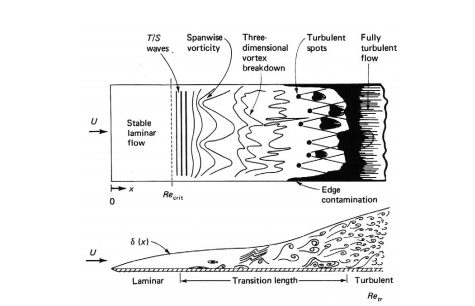
\includegraphics[scale=.7]{figures/boundary_layer_transition.png}
    \caption{This is the illustration of the transition from laminar to turbulent flow on the
    surface of an airplane. This transition is important in the design of a plane flying in
    Low Reynolds Number flow.}
  \label{fig:boundary_layer_transition}
\end{figure}

One aspect of the laminar boundary layer is the location in which it separates from the surface.
This transition region has many stages. At the first stage, unstable two-dimensional Tollmien Schlichting
waves are developed and start to move downstream. As it moves downstream, the waves become three directional
and vortical structures are formed. Finally this leads to turbulent flow.
Because of the instability this transition between turbulence and laminar flow 
can cause, predicting this location is important in the stability and other properties of the flight. 
This transition location also results in hysterisis effects. Before separation
occurs, increasing angle of attack will increase lift. But afterwards,
decreasing the angle of attack does not return to the same lift. 

One effect of laminar vs turbulence is the skin friction. When the flow is turbulent there
is a lot more skin friction then when it is laminar. The other side of it is, 
in terms of lift, maximum
lift depends on the characteristics of the turbulent boundary layer, because the
turbulent layer has the ability to recover pressure at the
rear of the airfoil.

Here are some Reynold number regimes for different boundary layers ~\cite{mueller}.

\begin{enumerate}
\item For Reynold numbers between 1000 and 10000 the boundary layer flow is laminar
and doesn't transition into trubulent flow. This type of flight is seen with
the dragon fly and the house fly. 
\item  For Reynold numbers between 10000 and 30000 the boundary layer is laminar but
it can separate. When it separates it does not reattach.
\item At 30000 to 70000 there are hysterisis effects because of the transition. 

\end{enumerate}

\subsection{Lateral Stability}

\subsubsection{Dihedral vs Anhedral}
\label{sec:dihedral}

Dihedral and anhedral refer to the angle between the wings and the horizontal plane.
Dihedral wings point upwards, and anhedral wings point
downwards as shown in Figure~\ref{fig:dihedraleffect}. Dihedral wings have more lateral 
stability than anhedral wings.

\begin{figure}[hl]
  \centering
    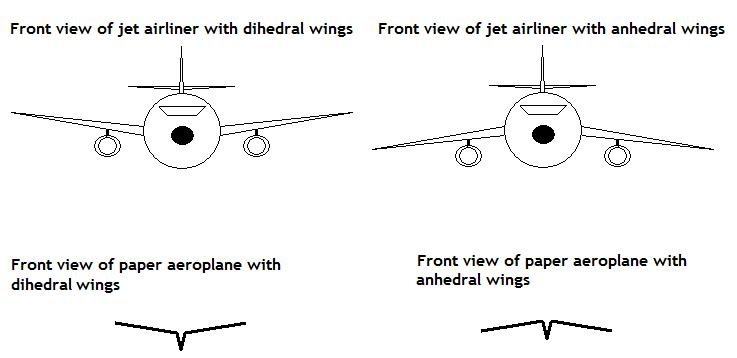
\includegraphics[scale=.5]{figures/dihedraleffect.png}
    \caption{A depiction between anhedral and dihedral wings}
  \label{fig:dihedraleffect}
\end{figure}

The bank angle is defined as the angle about the axis along
the plane's motion. Let us call the bank angle $\phi$. When the aircraft is
banked, this results in a rolling moment, called the dihedral effect. If the
rolling moment opposes the bank, the dihedral effect is positive. In order for
there to be stability, the dihedral effect needs to be positive. There are many
different factors that can contribute to the dihedral effect: the shape of the wings,
the wing placement, tail height, etc. We will analyze the angle of the wings in this paper.

To analyze this effect in more detail we will show that a dihedral aircraft has 
a positive dihedral effect. When the aircraft is banked we see that there is a net force
to the side, this is called sideslip (Figure~\ref{fig:dihedral1}). 
However we see that the forces on the wings do not 
contribute to the dihedral effect yet.


\begin{figure}[hl]
  \centering
    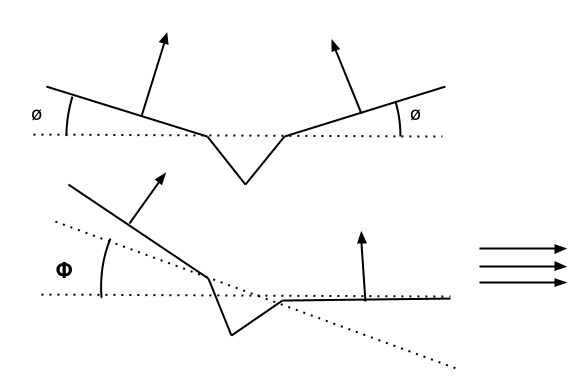
\includegraphics[scale=.5]{figures/dihedral1.png}
    \caption{An illustration of what happens when there is a lateral peturbation}
  \label{fig:dihedral1}
\end{figure}

At this point, with respect to the plane's frame of reference, there is air flowing 
to the side that will contribute to a dihedral effect. 
If the bank angle is $\phi$ and
the angle that the wings make with the horizontal is $\theta$ then after factoring in
the banked angle, the right wing has an angle of attack of  $\theta - \phi$.
The left wing has an angle of attack $- \theta - \phi$.
From our discussions of models of wings of airplane, we can say that the
coefficient of lift is approximately $\beta \sin(\alpha 0 \alpha_o)$.
$\alpha$ is the angle of attack and $\beta$ is a constant. To test the stability of the plane
let us assume that $|\phi| < |\theta|$.
So if we assume that $\theta$ is positive , so that the airplane is dihedral.
So the left wing will experience a downward force because of a negative angle of attack
and the right wing will experience an upwards force because of a positive angle of attack, straightning the plane out.
However, if $\theta$ is negative, and the plane is anhedral, the right wing will experience a
downwards force, and the left wing will experience an upwards force, increasing its lateral moment
(Figure~\ref{fig:dihedral2}). 


\begin{figure}[hl]
  \centering
    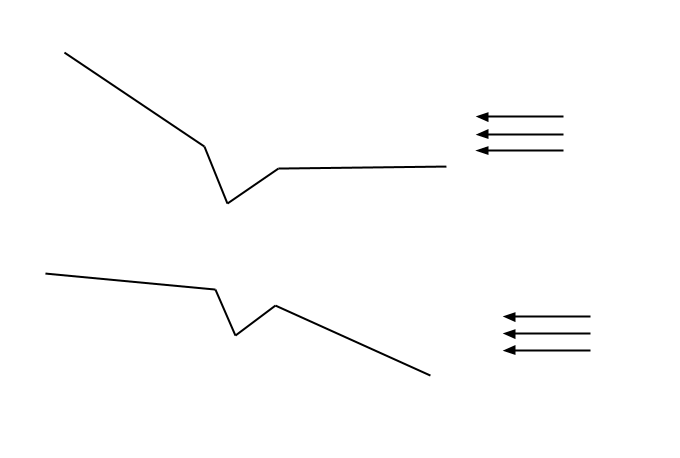
\includegraphics[scale=.5]{figures/dihedral2.png}
    \caption{A picture showing the difference between anhedral and dihedral wings. Dihedral wings offer 
    more lateral stability}
  \label{fig:dihedral2}
\end{figure}


\subsection{Longitudinal Stability}
\label{sec:long_stability}

\subsubsection{Aerodynamic Center}

The aerodynamic center is the location on the plane where the pitching moment doesn't
change with the angle of attack. 

In order to calculate it first we will show how to 
find moments at different locations given one moment. 
Let us say we know the moment of the plane, $M_{ref}$ at some
location $x_{ref}$. Also, as an approximation, we can also say that the upwards force
is the lift and the horizontal force is the drag. We would like to find the moment
at some $x_{new}$, $M_{new}$. Let us assume that the z dimension does not contribute to the
calculations because the airplane is pretty  is thin.

\[M_{ref} = -(x_{new} - x_{ref})L + M{new} \] 

because $-(x_{new} - x_{ref})L$ is the torque. We can convert this equation into their
respective coefficients, the pitching moment coefficient, and the lift coeffiient.

\[C_{m_{ref}} = - ( \frac{x_{new} - x_{ref}}{c})C_L + C_{m_{new}} \]

Where $c$ is the average chord length.

Next let us let $M_{new}$ be the moment about the aerodynamic center and
differentiate with respect to $\alpha$.

\[\od{C_{M_{ref}}}{\alpha} = - (\frac{x_{ac} - x_{ref}}{c}\od{C_L}{\alpha}) + (\od{C_{M_{ac}}}{\alpha})\].

By definition 
\[\od{C_{M_{ac}}}{\alpha} = 0\]

Therefore we can solve for $x_ac$ and we obtain:

\[\frac{x_{ac} - x_{ref}}{c} = \frac{x_{ref}}{c} - (\od{C_{M_{ref}}}{C_L})\]

Therefore, if we know the moment at one point, and we can figure out the derivative 
$\od{C_{M_{ref}}}{C_L}$. It has been found theoretically that this moment
occurs at a quarter of a chord back from the leading edge on most airfoils ~\cite{NASAac}.



\subsection{Wing Stability}
Let $\alpha$ be the angle with the horizontal. Also,
$C_M$ be the moment at the center of gravity.  In order for a plane to have static
stability

\begin{equation}
C_M = 0
\end{equation}
\begin{equation}
\od{C_M}{\alpha} < 0
\label{eq:long_stability}
\end{equation}

As we have shown in our models, the lift coeffient is a linear function of $\alpha$, therefore
we can conclude that the condition is

\[\od{C_M}{C_L} < 0 \]

To figure out the moment of the plane we start by figuring out the moment of the wings.
There are only two forces on the wings, the lift force and the drag force. Let us say
that the angle between the air flow and the airplane is $\alpha_{FRL}$ to the plane as shown in the picture below 
FIgure~\ref{fig:longitudinal_stability1}.

\begin{figure}[hl]
  \centering
    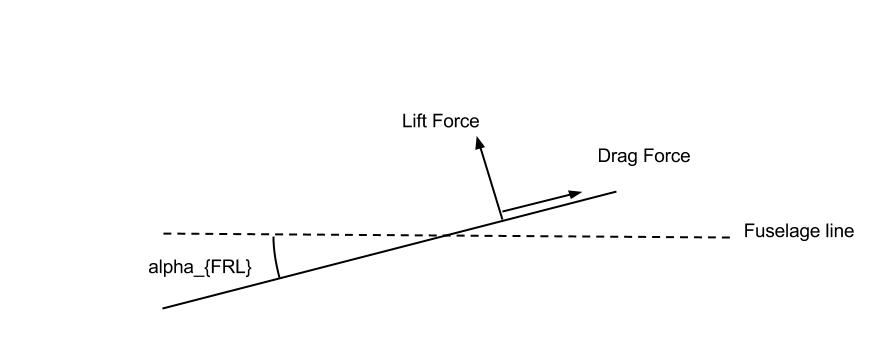
\includegraphics[scale=.5]{figures/longitudinal_stability1.png}
    \caption{An airplane is more stable if its center of gravity is closer to the nose of the plane than the
    aerodynamic center}
  \label{fig:longitudinal_stability1}
\end{figure}

From the formula from the previous section, we see that 

\[M_{cg}  = -(L\cos(\alpha_{FRL}) + D\sin(\alpha_{FRL}))(x_{cg} - x_{ac}) + M_{ac}\]

Again we will assume that the z component does not contribute. Then we change it into
coefficient form once more and use a small angle approximation.

\[ C_{M_{cg}} = -(C_{L} + C_D \alpha_{FRL}) (\frac{x_{cg}}{c} - \frac{x_{ac}}{c}) + C_{M_{ac}} \]

Because $\alpha_{FRL}$ is small we can approximate $C_{M_{cg}}$ as

\[-C_L (\frac{x_{cg}}{c} - \frac{x_{ac}}{c}) + C_{M_{ac}} \]

Because the aerodynamic center has no dependence on $\alpha_{FRL}$ we can rewrite the
stabiltiy equation as

\[\od{C_{M_{cg}}}{C_L} = - \frac{x_{cg}}{c} + \frac{x_{ac}}{c} < 0\]

Therefore, the bigger $x_{cg}$ is the more stable the plane is. By our choice of coordinate system,
this means that the center of mass of the plane has to be in front of the aerodynamic center for it to have
longitudinal stability.

              



\section{LAR wing Lift and Drag Models}

Low aspect ratio wings are wings where the ratio between the wing span and
the chord is small. Commertial aircrafts typically have high aspect ratio wings
to increase the amount of lift on the aircraft, but there are benefits of having
low aspect wings. Low aspect ratio aircrafts need to deal with less bending
stress because the wings are shorter. Also, the drag due to surface friction is
smaller because of the lower Reynold number from the bigger lengthscale.
For paper airplanes, low aspect ratio wings are definitely better than high
aspect ratio wings because paper can't overcome the
bending stress.


\subsection{Previous Research}

A lot of research about the lift and drag of wings with low aspect ratios  were done in the form of
micro-air vechicle research. This has the most relevance with paper airplanes because
micro-air vehicles operate on a Reynold number regime similar to paper airplanes. 
In 1999, Mueller showed that cambered plates offer better performance than flat plate wings, and
trailing-edge geometry does not have a strong effect on lift and drag
for thing wings at low Reynolds numbers. Also many experiments were done to experimentally
find the lift and drag coefficient of different wing shapes of different aspect ratios.

\subsection{Flat Plate model}

One way to model the wings is as a flat plane that is infinite in length. This corresonds to
an aspect ratio of zero. Since it is
an infinite flat plate, we can analyze it with a complex potential in two dimensions.
By means of conformal mapping, we can collapse a cylinder to a flat plate by

\[Z = z + \frac{a^2}{z}\].

\begin{figure}[hl]
  \centering
    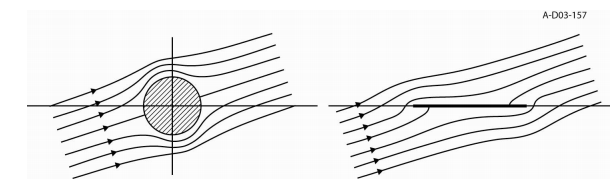
\includegraphics[scale=.5]{figures/flatplate1.png}
    \caption{An illustration of the conformal mapping from a cylinder to a flat plate. Figure adapted from ~\cite{thintheory}}
  \label{fig:dihedraleffect}
\end{figure}

Now let us consider a flow at an angle $\alpha$. A cylinder with a radius $r$
would result in a potential
\[w(z) = Ue^{i\alpha}(z + \frac{a^2}{z}) \]
After the conformal transformation, we see that the velocity now becomes
\[u - iv = \od{W}{Z} = \frac{\od{w}{z}}{\od{Z}{z}} = \frac{Ue^{-i\alpha}-Ue^{i\alpha}\frac{a^2}{z^2}
- \frac{i \Gamma}{2\pi z}}{1 - \frac{a^2}{z^2}}\]

In order to choose $\Gamma$ we must use the fact that the singularity at the trailing edge, 
$Z=2a$ or $z=a$ must be removed, from the Kutta condition. This condition occurs because 
a boundary layer prevents the flow from turning the sharp corner at the trailing edge.
The physical solution from complex flow theory depends on frictional forces.

Therefore we can find the circulation.

\[ \Gamma = -4\pi Ua \sin(\alpha) \]

This allows us to find the lift by the Kutta-Joukowski theorem.

\[L = \rho U \Gamma\]
\begin{equation}
\label{eq:flat_plat_cl}
C_L = 2\pi sin(\alpha)
\end{equation}

\subsection{Bollay Models}

The problem with the flat plate in the previous chapter is that it had to assume 
an aspect ratio of about zero in order to model it in that fashion. However, we can still
use the fact that the aspect ratio is small the model it in a similar fashion.
Let us assume that the wing is thin and has a low aspect ratio. Let the angle of attack
 be $\alpha$ and the velocity of the flow relative to the wing be $v$. 
 We can see that the normal component of the air
will have velocity $V\sin(\theta)$. Because the aspect ratio is low
we can model the flow around the wing like the flat plate model above.
This is depicted in Figure~\ref{fig:bollay1}

\begin{figure}[hl]
  \centering
    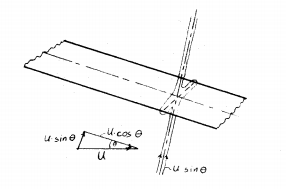
\includegraphics[scale=1]{figures/bollay1.png}
    \caption{An illustration of the flow around low aspect ratio wing. Figure adapted from~\cite{bollay}}
  \label{fig:bollay1}
\end{figure}


\[V\sin(\alpha)\]

If the angle is small enough this is approximately

\[V\alpha\]


It then follows that the lift force per unit length is just the normal velocity $V\alpha$ times the
rate of increase of a virtual additional mass. The virtual additional mass comes from the
added inertia from the fluid moving around the immersed object. From~\cite{jones} it is know that.

\begin{equation}
dm=\frac{\pi}{4}\rho b^2 dx
\end{equation}

If $\rho$ is the density of the fluid and $b$ and $x$ are the dimensions of the plate.

\[l = V\alpha \od{m}{t} = V^2\alpha \od{m}{x} \]

\[l = \pi \alpha \frac{\rho}{2}V^2 b \od{b}{x} \dif{x} \]

\[l = \pi \alpha \frac{\rho}{2} V^2 b \dif{b} \]

To get the entire lift force we can just integrate across the width of the wake. 

\[L = \frac{\pi \alpha \rho V^2 b_{max}}{4} \]

This results in a lift coefficient $C_L$ of

\begin{equation}
 \frac{\pi}{2} \AR \alpha 
 \label{eq:bollay_model}
 \end{equation}

Where $\AR$ is the aspect ratio. In the experiments section we will test whether or not the aspect ratio
would actually affect the lift coefficient.





%\appendix
%\chapter{Tables}

\begin{table}
\caption{Armadillos}
\label{arm:table}
\begin{center}
\begin{tabular}{||l|l||}\hline
Armadillos & are \\\hline
our	   & friends \\\hline
\end{tabular}
\end{center}
\end{table}

\clearpage
\newpage

%\chapter{Figures}

\vspace*{-3in}

\begin{figure}
\vspace{2.4in}
\caption{Armadillo slaying lawyer.}
\label{arm:fig1}
\end{figure}
\clearpage
\newpage

\begin{figure}
\vspace{2.4in}
\caption{Armadillo eradicating national debt.}
\label{arm:fig2}
\end{figure}
\clearpage
\newpage

%% This defines the bibliography file (main.bib) and the bibliography style.
%% If you want to create a bibliography file by hand, change the contents of
%% this file to a `thebibliography' environment.  For more information 
%% see section 4.3 of the LaTeX manual.
\begin{singlespace}
\nocite{*}
\bibliography{main}
\bibliographystyle{plain}
\end{singlespace}

\end{document}

